%% Преамбула TeX-файла

% 1. Стиль и язык
\documentclass[utf8x, 12pt]{G7-32} % Стиль (по умолчанию будет 14pt)


% Остальные стандартные настройки убраны в preamble.inc.tex.
\sloppy

% Настройки стиля ГОСТ 7-32
% Для начала определяем, хотим мы или нет, чтобы рисунки и таблицы нумеровались в пределах раздела, или нам нужна сквозная нумерация.
\EqInChapter % формулы будут нумероваться в пределах раздела
\TableInChapter % таблицы будут нумероваться в пределах раздела
\PicInChapter % рисунки будут нумероваться в пределах раздела

% Добавляем гипертекстовое оглавление в PDF
\usepackage[
bookmarks=true, colorlinks=true, unicode=true,
urlcolor=black,linkcolor=black, anchorcolor=black,
citecolor=black, menucolor=black, filecolor=black,
]{hyperref}

% Изменение начертания шрифта --- после чего выглядит таймсоподобно.
% apt-get install scalable-cyrfonts-tex

\IfFileExists{cyrtimes.sty}
    {
        \usepackage{cyrtimespatched}
    }
    {
        % А если Times нету, то будет CM...
    }

\usepackage{graphicx}   % Пакет для включения рисунков
\DeclareGraphicsExtensions{.jpg,.pdf,.png}
% С такими оно полями оно работает по-умолчанию:
% \RequirePackage[left=20mm,right=10mm,top=20mm,bottom=20mm,headsep=0pt]{geometry}
% Если вас тошнит от поля в 10мм --- увеличивайте до 20-ти, ну и про переплёт не забывайте:
\geometry{right=20mm}
\geometry{left=30mm}



% Произвольная нумерация списков.
\usepackage{enumerate}
\usepackage{enumitem}
\usepackage{amsmath}
\DeclareMathOperator*{\argmax}{arg\,max}

\setcounter{tocdepth}{1} %Подробность оглавления
%4 это chapter, section, subsection, subsubsection и paragraph
%3 это chapter, section, subsection и subsubsection
%2 это chapter, section, и subsection
%1 это chapter и section
%0 это chapter.


\begin{document}

\frontmatter % выключает нумерацию ВСЕГО; здесь начинаются ненумерованные главы: реферат, введение, глоссарий, сокращения и прочее.
\begin{center}
РЕФЕРАТ
\end{center}

% \large Московский авиационный институт\\[5.5cm]

% \huge Реферат \\[0.6cm] % название работы, затем отступ 0,6см
% \large на тему:  <<Метод идентификации музыкальных
% произведений по аудио фрагментам концертных исполнений>>\\[3.7cm]


% \end{center}

% \begin{flushright}
% Выполнил: студент гр. М8О-406Б \\
% Давид Гринберг \\
% \end{flushright}


% \vfill

% \begin{center}
% \large Москва 2020
% \end{center}

% \thispagestyle{empty}
Выпускная квалификационная работа содержит \pageref{LastPage} страницу, \totfig{}
рисунков, \total{citnum}\ использованных источников.

АКУСТИЧЕСКИЙ ОТПЕЧАТОК, ИНФОРМАЦИОННЫЙ ПОИСК, МЕТОД ГЛАВНЫХ КОМПОНЕНТ, SHAZAM, МУЗЫКАЛЬНЫЙ АНАЛИЗ, ВРЕМЕННЫЕ РЯДЫ.

Выпускная квалификационная работа посвящена разработке библиотеки создания акустических оптечатков с помощью
алгоритма, основанного на методе главных компонент и решению с ее помощью задачи идентификации музыкальных произведений
по аудио фрагментам концертных исполнений.

В теоретической части рассматриваются общие подходы к хранению и поиску аудиофайлов, описывается алгоритм
создания акустических отпечатков. Также предлагаются способы оптимизации поиска аудифайлов.

В практической части рассматривается архитектура реализованной библиотеки, приводятся результаты замеров
ее эффективности. Кроме того, описывается дальнейшее развитие библиотеки.


\thispagestyle{empty}
\setcounter{page}{0}
\setcounter{tocdepth}{2}
\setcounter{secnumdepth}{2}
\tableofcontents
\clearpage


\Introduction

В современном мире наблюдаются следующие тенденции:
\begin{itemize}
    \item Люди нетерпеливы и привыкли к легкому и быстрому доступу к информации
    \item Количество доступной информации неукротимо растет и человек не в состоянии
    справиться с ее потоком без использования поисковиков
    \item Существенная часть информации -- аудиофайлы
\end{itemize}

Конкретный пример: люди, посещающие различные музыкальные мероприятия, часто сталкиваются
с ситуацией, когда на сцене выступает музыкант, а название песни
или даже имя исполнителя неизвестно (например, на фестивале).
Конечно, можно спросить ближайшего человека, но в таких местах обычно очень шумно.
Кроме того нет гарантий, что у этого человека найдется ответ на вопрос.
Существует множество методов и сервисов для нахождения музыкальных произведений по отрывку,
однако у них есть ряд ограничений:
\begin{itemize}
    \item Сервисы вроде Shazam способны распознавать только оригиналы
    \item Некоторые сервисы умеют искать произведения по мелодии, но у них
            довольно низкая точность.
    \item Сервисы, которые ищут каверы или ремиксы (для защиты авторских прав) не приспособлены
            к нахождению зашумленных отрывков, поскольку предполагают, что кавер записывался в
            студийных условиях
\end{itemize}
В этой работе рассмотрен метод, лишенный всех вышеобозначенных недостатков.
Поскольку музыкальных произведений в мире очень много (например, в социальной сети VK 400 миллионов треков),
то очень важно уметь быстро и эффективно по памяти обрабатывать эти данные.
Кроме того этот метод применим не только к песням, так как аудиофайл представляет собой временной ряд.\\
Цели данной работы:
\begin{enumerate}[label=\arabic*.]
    \item Разработать библиотеку, которая предоставляла бы гибкий и удобный интерфейс
            для эффективной обработки и поиска аудиофайлов
    \item Реализовать клиент для идентификации концертных записей, используя разработанную
    библиотеку
\end{enumerate}


\mainmatter

\chapter{Теоретическая часть}
\label{cha:ch_1}

\section{Звук}
Звук - это вибрация, которая распространяется через воздух (или воду).
Например, при прослушивании музыки с компьютера колонки производят вибрации,
которые распространяются по воздуху, пока не достигнут уха человека.

Вибрации можно смоделировать с помощью синусоидальных волн.

\subsection{Чистый тон}
Чистый тон - это тон синусоидальной формы волны. Характеристики синусоиды:
\begin{itemize}
    \item Частота: количество циклов в секунду. Единица измерения - Герц (Гц), например, 100 Гц = 100 циклов в секунду.
    \item Амплитуда (связана с громкостью звука): размер каждого цикла.
\end{itemize}

Эти характеристики расшифровываются человеческим ухом для формирования звука.
Человек может слышать чистые тоны от $20$ Гц до $20 000$ Гц,
и этот диапазон уменьшается с возрастом. Для сравнения, свет, который видит человек,
состоит из синусоид от $4 * 10^{14}$ Гц до $7.9 * 10^{14}$ Гц.

Человеческое восприятие громкости зависит от частоты чистого тона.
Например, чистый тон с амплитудой равной $10$ и частотой $30$ Гц будет тише,
чем чистый тон с амплитудой $10$ и частотой $1000$ Гц.
Человеческие уши воспринимают звук в соответствии с психоакустической моделью.

Чистых тонов в природе не существует, однако каждый звук в мире - это сумма
нескольких чистых тонов с разными амплитудами.

\subsection{Музыкальные ноты}
Ноты разделены на октавы. В большинстве западных стран октава представляет
собой набор из 8 нот (A, B, C, D, E, F, G в большинстве англоязычных
стран) со следующим свойством:
\begin{itemize}
    \item Частота ноты в октаве удваивается в следующей октаве.
    Например, частота А4 (А в 4-й октаве) на частоте 440 Гц в 2 раза
    превышает частоту А3 (А в 3-й октаве) на 220 Гц и в 4 раза больше
    частоты А2 (А во 2-й октаве) на 110 Гц.
\end{itemize}

% Для 4-й октавы ноты имеют следующую частоту:
% \begin{itemize}
%     \item C4 = 261.63 Гц
%     \item D4  = 293.67 Гц
%     \item E4 = 329.63 Гц
%     \item F4 = 349.23 Гц
%     \item G4 = 392 Гц
%     \item A4 = 440 Гц
%     \item B4 = 493.88 Гц
% \end{itemize}

Частотная чувствительность ушей логарифмическая. Это означает, что:
\begin{itemize}
    \item между 32.70 Гц и 61.74 Гц (1-я октава)
    \item или между 261.63 Гц и 466.16 Гц (4-я октава)
    \item или между 2 093 Гц и 3 951.07 Гц (7-я октава)
\end{itemize}

Человеческие уши распознают одинаковое количество нот.

\subsection{Тембр}
Одна и та же нота может звучать по-разному, если ее играют гитара, пианино или скрипка.
Причина в том, что у каждого инструмента свой тембр для данной ноты.

Для каждого инструмента воспроизводимый звук представляет собой множество частот,
которые звучат как данная нота (научный термин для музыкальной ноты - высота звука).
Этот звук имеет основную частоту (самая низкая частота) и несколько обертонов (любая частота выше основной).

Большинство инструментов производят гармоничные звуки.
Для этих инструментов обертоны являются кратными основной частоты и называются гармониками.
Например, композиция чистых тонов A2 (основной), A4 и A6 является гармонической,
тогда как композиция чистых тонов A2, B3, F5 является негармоничной.

Многие ударные инструменты (например, тарелки или барабаны) создают негармоничные звуки.

Примечание: высота звука (воспринимаемая музыкальная нота) может отсутствовать в звуке,
воспроизводимом инструментом. Например, если инструмент воспроизводит звук с чистыми
тонами A4, A6 и A8, человеческий мозг интерпретирует полученный звук как ноту A2.
Эта нота / высота звука будет A2, тогда как самая низкая частота звука - A4
(этот факт называется отсутствующим основным).

\subsection{Цифровое представление звука}
Чтобы хранить и проигрывать звук на электронных устройствах, его нужно оцифровать.

\subsubsection{Семплирование}
Аналоговые сигналы - это непрерывные сигналы, что означает, что если взять одну секунду
аналогового сигнала, то ее можно разделить на части, которые длятся доли секунды.
В цифровом мире нельзя позволить себе хранить бесконечное количество информации.
Нужно иметь минимальную единицу времени, например, 1 миллисекунду.
В течение этого промежутка времени звук не сможет измениться, поэтому этот промежуток должен быть
достаточно коротким, чтобы цифровой сигнал звучал как аналоговый, и достаточно большой,
чтобы ограничить пространство, необходимое для хранения.

Эта задача называется семплированием.
\begin{figure}[H]
    \begin{center}
        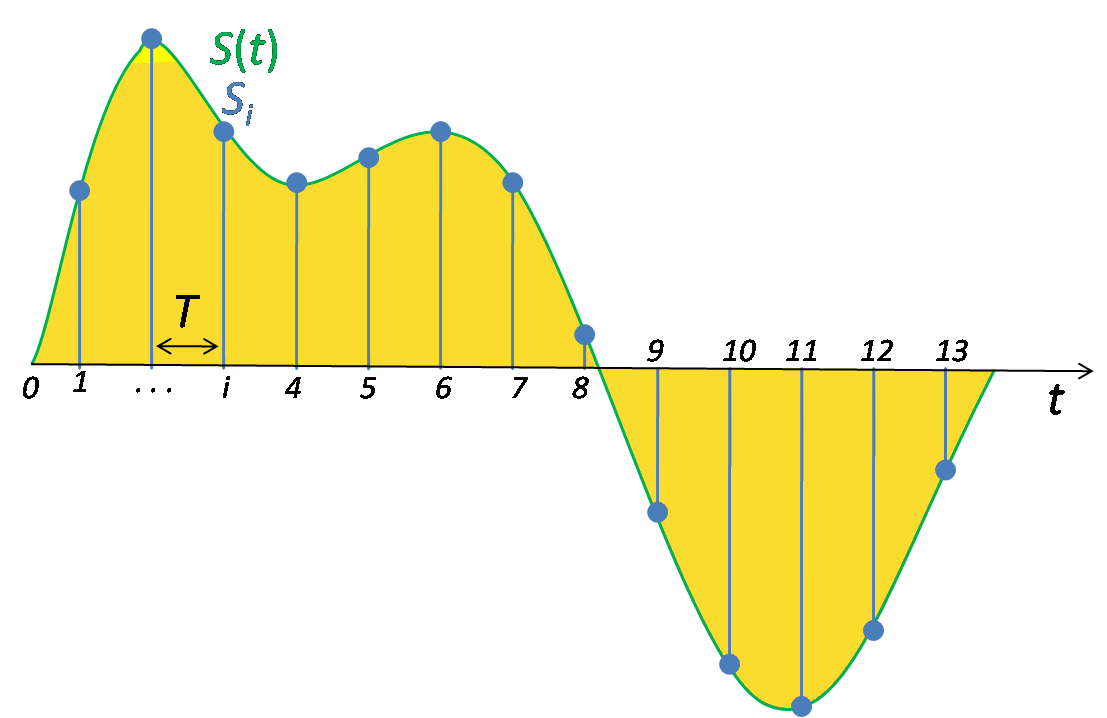
\includegraphics[scale=0.3]{inc/img/Signal_Sampling.png}
        \caption{Пример семплирования}
    \end{center}
\end{figure}

Стандартная единица времени в цифровой музыке составляет 44100 единиц (или сэмплов) в секунду.
Эта величина выбрана в связи с теоремой Котельникова, из которой следует,
что для оцифровки синусоиды частоты $F$ требуется, по меньшей мере, 2 точки на цикл.
Так как человек слышит в пределах 20 кГц, то соответственно для оцифровки сигналов нужно использовать
вдвое больше точек.

\subsubsection{Квантизация}
Громкость измеряет разницу между самым
низким и самым высоким уровнем звука в песне.
Как и в случае с семплированием, для оцифровки сигнала требуется иметь ограниченное количество
уровней громкости.

Эта задача называется квантизацией.
\begin{figure}[H]
    \begin{center}
        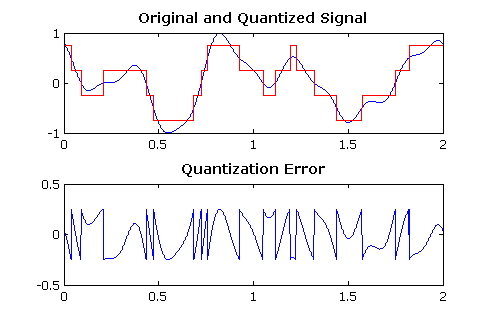
\includegraphics[scale=0.7]{inc/img/Quanterr.png}
        \caption{Пример квантизации}
    \end{center}
\end{figure}

\subsection{Спектрограмма}
Музыкальное произведение исполняется несколькими инструментами и певцами.
Все эти инструменты производят комбинацию синусоидальных волн на нескольких частотах,
и в целом комбинация синусоидальных волн еще больше.

Можно визуализировать музыку с помощью спектрограммы.
В большинстве случаев спектрограмма представляет собой трехмерный график, где:
\begin{itemize}
    \item по оси X представлено время (точнее его промежуток),
    \item по оси Y представлена частота чистого тона
    \item третье измерение описывается цветом и соответствует амплитуде частоты в определенное время.
\end{itemize}

\begin{figure}[H]
    \begin{center}
        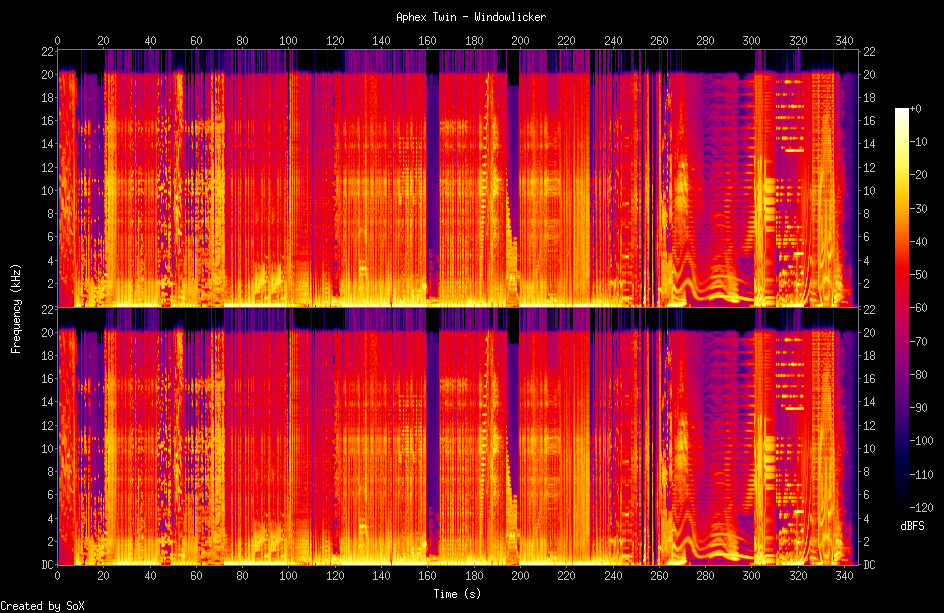
\includegraphics[scale=0.4]{inc/img/windowlicker.png}
        \caption{Спектрограмма Aphex Twin -- Windowlicker}
    \end{center}
\end{figure}

\subsection{Дискретное преобразование Фурье}
Для того, чтобы вычислить спектрограмму дискретного сигнала, нужно найти
его частоты. Это можно сделать с помощью дискретного преобразования Фурье (ДПФ).
ДПФ применяется к дискретным сигналам и его результатом является дискретный спектр (частоты внутри сигнала).

Формула ДПФ:
$$X(n) = \sum_{k=0}^{N-1} x(k) \times e^{-i \frac{2 \pi n k}{N}}$$,
где $N$ -- размер окна (количество семплов),
$X(n)$ -- $n$-ый диапазон частот,
$x(k)$ -- $k$-ый семпл сигнала

\section{Техника акустического отпечатка}
Для того, чтобы эффективно хранить и искать аудиофайлы, нужно
найти какое-нибудь компактное представление, которое при этом будет
максимально правдоподобно их описывать.
Это представление называется акустическим отпечатком (фингерпринтом) аудиофайла.
Существует множество видов таких отпечатков, но большинство методов
находят представление аудиофайлов в виде вектора хешей.

Факторы эффективности:
\begin{enumerate}[label=\arabic*.]
    \item Хеши максимизируют произведение функций энтропии и точности:
    \begin{figure}[H]
        \begin{center}
            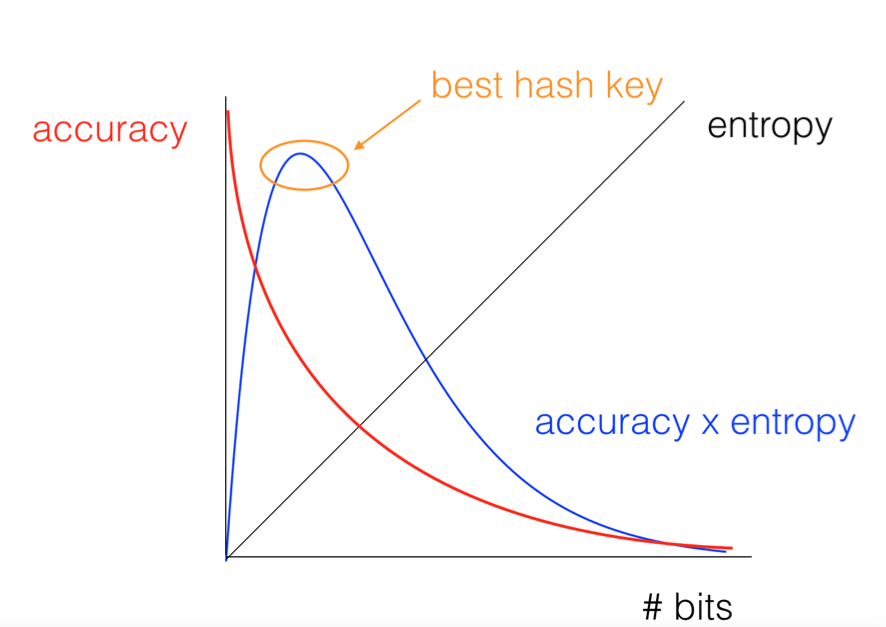
\includegraphics[scale=0.6]{inc/img/best_hp.png}
            \caption{Зависимость эффективности от точности и энтропии}
        \end{center}
    \end{figure}
    \item Биты хешей сбалансированы, декоррелированы и имеют высокую дисперсию
\end{enumerate}

\subsection{Общая идея}
Многие алгоритмы фингерпринтинга выглядят так:
\begin{enumerate}[label=\arabic*.]
    % \item Индексация:
    % \begin{enumerate}
        \item Посчитать спектрограмму аудиофайла
        \item Применить на ней какую-либо оконную функцию (спектрально-временные фильтры)
        \item Конвертировать результат в вектор хешей
    %     \item Посчитать обратный индекс вида:
    %     $$hash \to [... \{song\_id,\ offset\} ... ]$$, где $offset$ -- это
    %     номер временного диапазона аудиофайла, соответствующего $song\_id$,
    %     в котором встречается $hash$.
    % \end{enumerate}
    % \item Поиск:
    % \begin{enumerate}
    %     \item Посчитать акустический отпечаток запроса
    %     \item Поскольку
    % \end{enumerate}
\end{enumerate}

\section{Метод хешпринтов}
Этот метод предложен в \cite{tsai}. Он, как и многие другие, находит представление
аудиофайла в виде вектора хешей.

Метод отличается следующими характеристиками:
\begin{enumerate}[label=\arabic*.]
    \item Обучение без учителя
    \item Высокая адаптивность к данным
    \item Независимость от силы сигнала (громкости звука)
\end{enumerate}

Самой важной отличительной чертой метода является обучение без учителя.
Такие методы, как, например, Chromaprint, описанный в \cite{chromaprint}, используют
заранее подготовленные спектрально-временные фильтры.
Метод хешпринтов находит эти фильтры непосредственно при индексации, что позволяет
ему учитывать специфику данных.
\begin{figure}[H]
    \begin{center}
        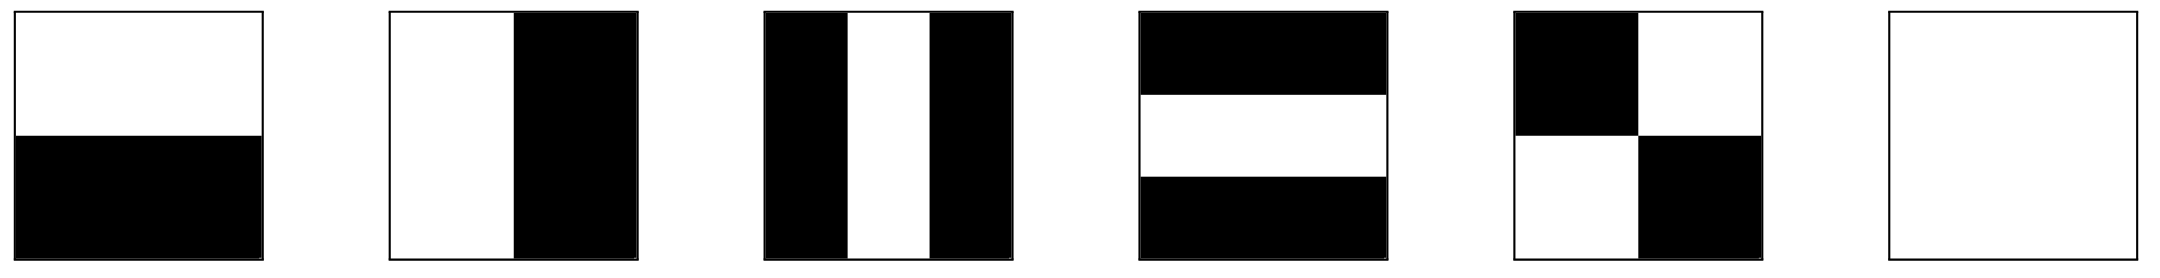
\includegraphics[scale=0.3]{inc/img/chroma.png}
        \caption{Фильтры, используемые Chromaprint}
    \end{center}
\end{figure}

\subsection{Алгоритм вычисления хешпринта}
Для вычисления хешпринта, содержащего $N$ бит, нужно проделать следующее:
\begin{enumerate}[label=\arabic*.]
    \item Посчитать спектрограмму.\\
    Результат этапа: матрица $Spectrogram \in \mathbb{R}^{B \times n}$, где $B$ -- количество частотных диапазонов,
    \begin{figure}[H]
        \begin{center}
            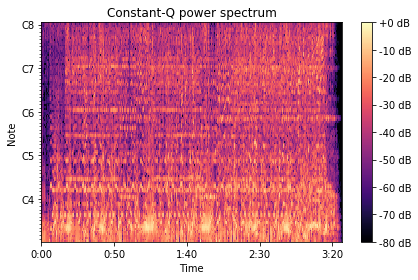
\includegraphics[scale=0.6]{inc/img/spectrogram.png}
            \caption{Спектрограмма}
        \end{center}
    \end{figure}
    $n$ -- количество временных диапазонов.
    \item Собрать контекстные фреймы полученной спектрограммы.
    Фреймы рассчитываются следующим образом:
    $$frame_i = V_{i-w}...V_{i+w}$$, где $V_i$ -- столбец спектрограммы, $w$ -- количество столбцов контекста.\\
    Результат этапа: матрица $Frames \in \mathbb{R}^{Bw \times n}$
    \begin{figure}[H]
        \begin{center}
            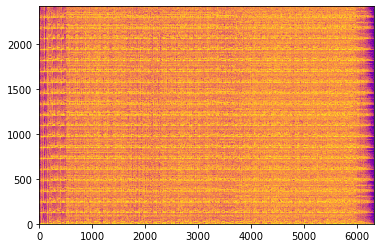
\includegraphics[scale=0.6]{inc/img/frame.png}
            \caption{Матрица фреймов}
        \end{center}
    \end{figure}
    \item Применить к фреймам спектрально-временные фильтры. Фильтры представляют собой
    $N \times Bw$ матрицу и расситываются c помощью алгоритма обучения без учителя
    путем решения задачи оптимизации.\\
    Результат этапа: матрица признаков $Features \in \mathbb{R}^{N \times n}$.
    \begin{figure}[H]
        \begin{minipage}{.5\textwidth}
            \centering
            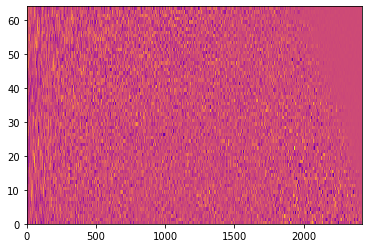
\includegraphics[scale=0.6]{inc/img/filters.png}
            \caption{Фильтры}
        \end{minipage}%
        \begin{minipage}{.5\textwidth}
            \centering
            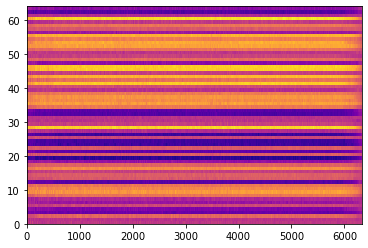
\includegraphics[scale=0.6]{inc/img/features.png}
            \caption{Матрица признаков}
        \end{minipage}
    \end{figure}
    \item Посчитать дельту -- изменение признаков в течение промежутка $T$.
    Дельта рассчитывается по формуле:
    $$\Delta_i = feature_i - feature_{i+T}$$
    \begin{figure}[H]
        \begin{center}
            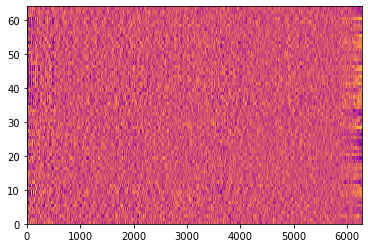
\includegraphics[scale=0.6]{inc/img/delta.png}
            \caption{Дельта}
        \end{center}
    \end{figure}
    \item Наложить функцию порога и упаковать результат в хешпринты:
    $$hashprint_i = intN(\Delta_i > 0)$$
    \begin{figure}[H]
        \begin{center}
            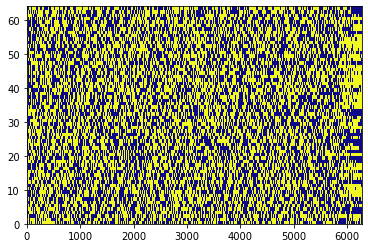
\includegraphics[scale=0.6]{inc/img/thres.png}
            \caption{Результат наложения функции порога}
        \end{center}
    \end{figure}
\end{enumerate}

\subsection{Вычисление спектрально-временных фильтров}
Фильтры подбираются таким образом, чтобы признаки, полученные при их наложении,
имели максимальную дисперсию и в то же время были декоррелированы.\\
Для этого можно применить метод главных компонент (PCA):
\begin{enumerate}[label=\arabic*.]
    \item Посчитать ковариационные матрицы для всех матриц фреймов в базе
    и просуммировать их.\\
    Результат этапа: матрица $CovarianceMatrix \in \mathbb{R}^{Bw \times Bw}$
    \item Найти $N$ собственных векторов с максимальными собственными значениями.\\
    Результат этапа: матрица $Filters \in \mathbb{R}^{N \times Bw}$
\end{enumerate}

\section{Задача идентификации живых отрывков}
Поскольку речь идет о нечетком поиске, то мы хотим учесть как можно
больше нюансов (признаков) сигнала. Поэтому будем представлять аудиофайлы в виде
64-битных хешпринтов. Также в качестве спектрограммы возьмем CQT спектрограмму -
она хороша тем, что ее частотные диапазоны подобраны таким образом, что они
соответствуют конкретным нотам.

\subsection{Хранение и поиск}
У живого исполнения с большой долей вероятности будет много общих признаков
в определенные моменты времени со студийным оригиналом. Также мы знаем, что
если какой-то аудиофайл является отрывком другого, то это значит что существует
такой отступ $offset$, что $fragment \approx original[offset..]$.

Таким образом, задача обретает вид:
$$ans = \argmin_{original, offset}d(fragment, original[offset..])$$,
где $d$ -- некоторая метрика. Проще говоря, мы хотим минимизировать расстояние между
отрывком и студийным оригиналом. Также стоит отметить, что такой подход подразумевает,
что музыкант не сильно изменил темп исполнения по сравнению с оригиналом.

\subsection{Почему обратный индекс не подходит}
Хранение и поиск аудиофайлов можно было бы организовать следующим образом:
\begin{enumerate}[label=\arabic*.]
    \item Построим обратный индекс вида:
    $$hashprint \to [...\{song\_id, offset\}...]$$
    \item Заводим счетчик. Для каждого хешпринта отрывка
    найдем все пары $\{song\_id, offset\}$, в которых содержатся
    соответствующие хешпринты и увеличим для них счетчик.
    \item Возвращаем пару с максимальным значением счетчика.
\end{enumerate}
У такого подхода есть одна проблема. Мы имеем дело с пространством довольно
большой размерности и вероятность того, что в отрывке и оригинале в один момент времени
встретятся полностью одинаковые хешпринты очень мала.

\subsection{Вариант авторов метода}
В качестве метрики берется сумма расстояний Хемминга между соответствующими хешпринтами
при прикладывании отрывка к оригиналу.
Также подразумевается, что есть некий сервис, который по GPS определит
ближайший концерт и соответственно исполнителя, что позволит проверить лишь малую часть базы.\\
Сам же поиск выглядит так:
\begin{enumerate}[label=\arabic*.]
    \item Для каждого оригинала из базы: прикладываем к нему отрывок и ищем такой отступ, чтобы сумма расстояний
    Хемминга между соответствующими хешпринтами была минимальной.
    \begin{figure}[H]
        \begin{center}
            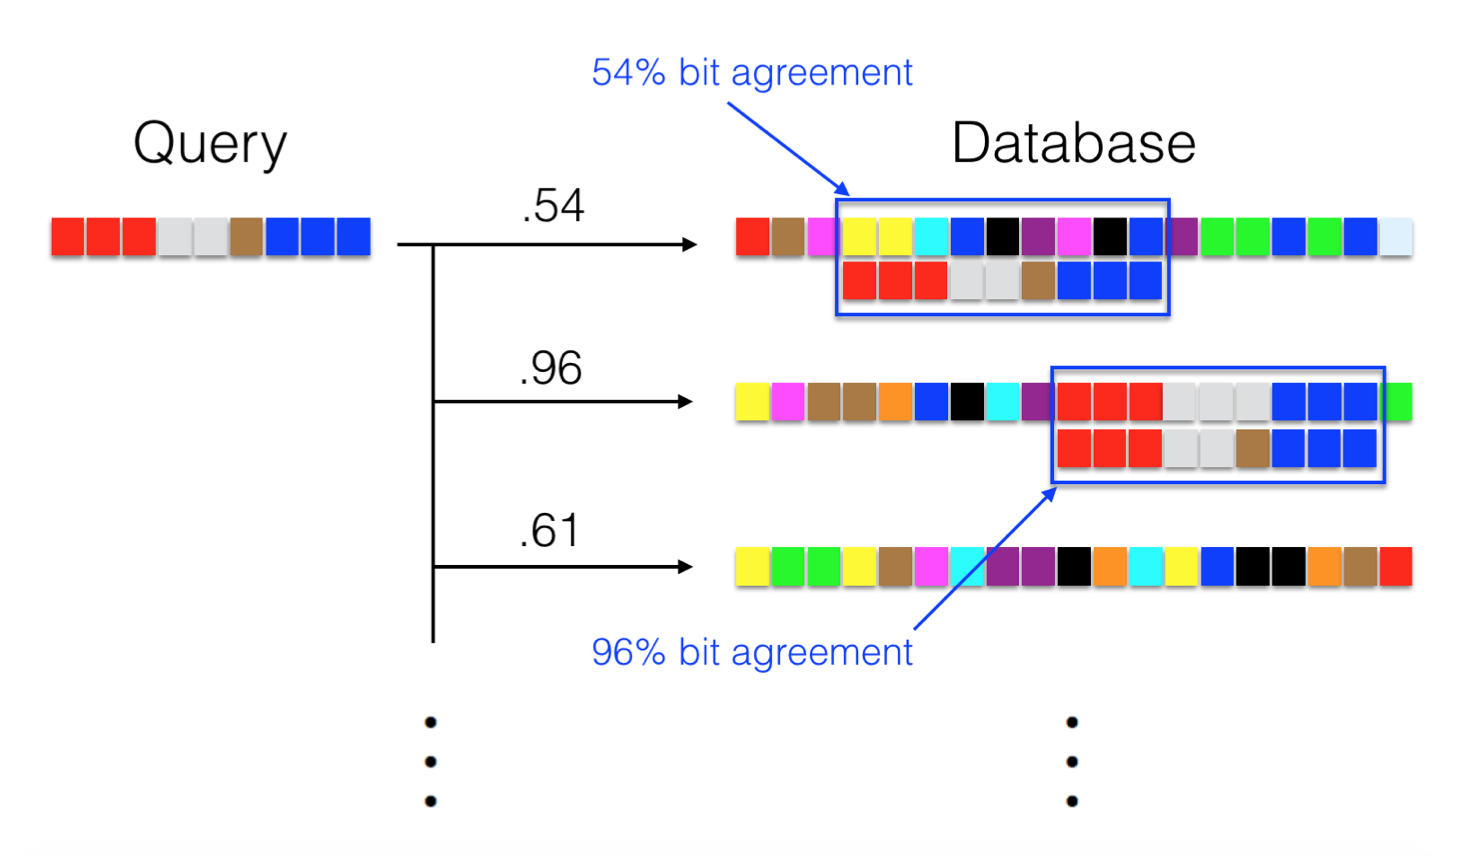
\includegraphics[scale=0.5]{inc/img/query.png}
            \caption{Пример обработки запроса}
        \end{center}
    \end{figure}
    \item Собираем результаты, сортируем и возвращаем top-N.
\end{enumerate}

Минус такого подхода -- GPS сервис:
\begin{enumerate}[label=\arabic*.]
    \item Точка отказа. Упадет сервис -- упадет вся система
    \item Затраты на разработку и поддержку сервиса
    \item Если это внешний сервис, то первый пункт становится еще большей проблемой
\end{enumerate}

Конечно, чаще всего человек знает на чей концерт он пришел и нужды в GPS сервисе не будет.
С другой стороны в наше время наблюдается рост числа музыкантов (по крайней мере в России),
поскольку делать музыку и делиться ей стало легче чем когда-либо.
Многие из этих музыкантов неизвестны широкому кругу слушателей, и они не готовы тратить
деньги на рекламу своего творчества, но периодически выступают на различных концертах
и фестивалях, где публика их возможно не узнает.

Но главная проблема в том, что этот метод имеет большой потенциал для применения
в других областях (например, классификация ЭКГ), в которых GPS сервис никак не поможет.
Чтобы сократить время поиска, нужно научиться каким-то образом отсекать большую часть данных.

\subsection{Метод k-ближайших соседей}
Можно взять вариант поиска с обратным индексом и заменить обратный индекс на
поиск k-ближайших соседей. Нам не критично, чтобы находились абсолютно все ближайшие соседи,
поэтому можно использовать методы приближенного поиска ближайших соседей
(approximate nearest neighbor), у которых выше производительность.

Мною было рассмотрено два алгоритма:
\begin{itemize}
    \item Метод случайных проекций.
    \item Иерархический маленький мир (HNSW)
\end{itemize}

Лучше всего себя показал HNSW.

\subsubsection{Метод случайных проекций}
Разбивает пространство гиперплоскостями и строит несколько бинарных деревьев.
Реализация: \href{https://github.com/spotify/annoy}{annoy}
\begin{itemize}
    \item[$-$] Производительность хуже, чем у другого алгоритма
    \item[$-$] Требует много памяти
\end{itemize}

\begin{figure}[H]
    \centering
    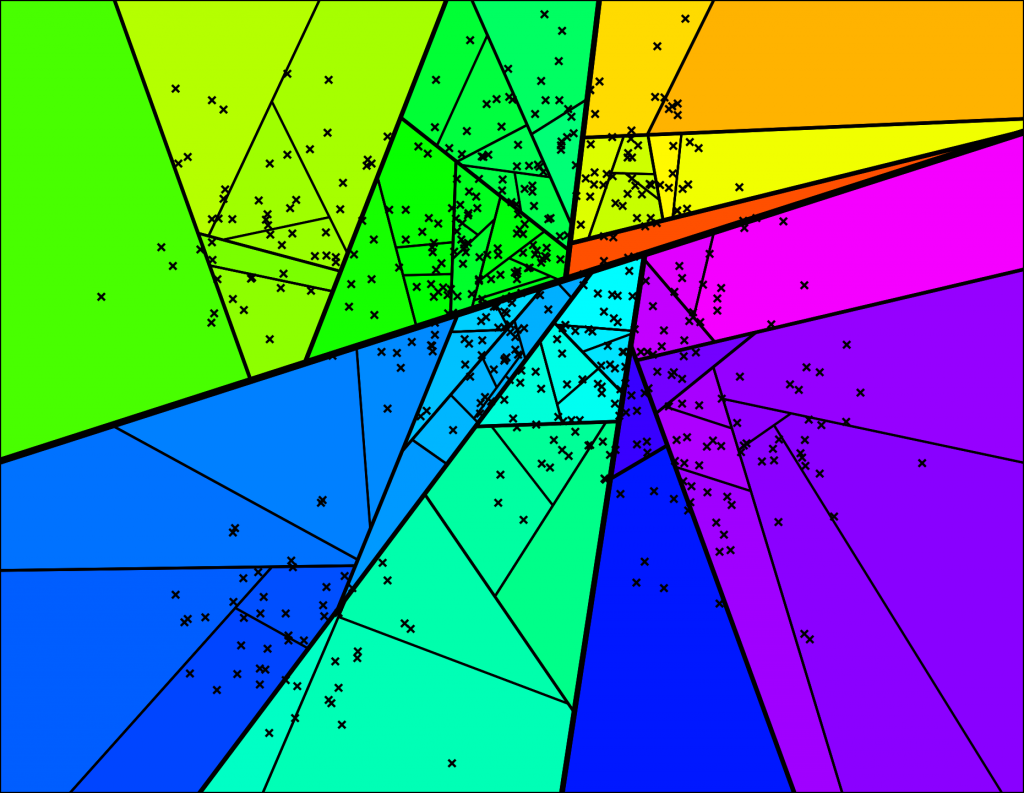
\includegraphics[scale=0.5]{inc/img/annspace.png}
    \caption{Пространство, разбитое гиперплоскостями}
\end{figure}

\begin{figure}[H]
    \centering
    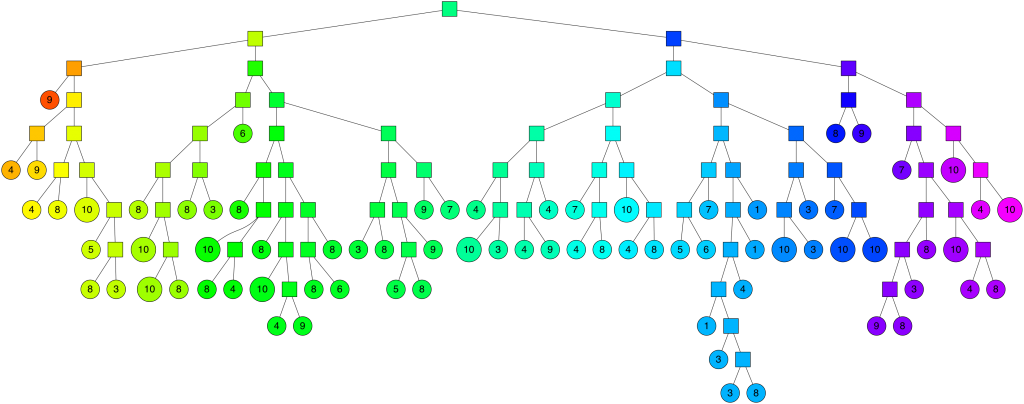
\includegraphics[scale=0.57]{inc/img/anntree.png}
    \caption{Соответствующее разбиению бинарное дерево}
\end{figure}

\subsubsection{Иерархический маленький мир}
Граф <<мир тесен>> -- это такой граф, в котором типичное расстояние $L$ между двумя
произвольно выбранными вершинами растёт пропорционально логарифму от числа
вершин: $L \propto \log{N}$.

В библиотеке \href{https://github.com/nmslib/nmslib}{nmslib} реализован алгоритм HNSW,
описанный в \cite{hnsw}. HNSW совмещает в себе свойства графа <<мир тесен>> и списка с пропусками.
По сути это иерархия графов, которая состоит из $n$ слоев: на нулевом слое представлены
все объекты, а по мере увеличения слоя -- все меньшая и меньшая их подвыборка.
При этом все объекты на слое $n+1$ есть и на слое $n$.
\begin{figure}[H]
    \begin{center}
        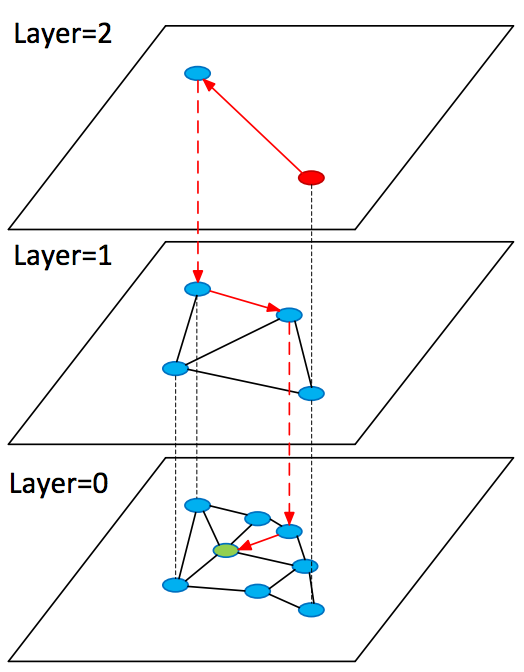
\includegraphics[scale=0.4]{inc/img/hnsw.png}
        \caption{Пример графа}
    \end{center}
\end{figure}

При поиске старт происходит со случайной вершины в графе верхнего слоя, там мы быстро
находим близкие к запросу вершины и возобновляем поиск с них на предыдущем слое.


Алгоритм очень легко масштабируется -- можно сделать ребро между вершинами, находящимися
на разных физических машинах. Также у HNSW хорошая производительность и небольшие затраты
на память.
\chapter{Практическая часть}
\label{cha:ch_2}

В рамках ВКР была реализована
библиотека hpfw (\href{https://github.com/kisasexypantera94/hpfw}{\color{blue} ссылка} на Github).
С использованием инструментов библиотеки была решена задача идентификации музыкальных
произведений по фрагментам концертных исполнений. Для этой же
задачи написан Telegram-бот (\href{https://t.me/hpfw_bot}{\color{blue} ссылка} на бота).

\section{Технологии}
В библиотеке hpfw используются:
\begin{itemize}
    \item C++17
    \item essentia -- для вычисления спектрограмм
    \item Eigen3 -- для линейной алгебры
    \item cpp-taskflow -- для распараллеливания индексации
\end{itemize}

Для библиотеки также написан Python-клиент.

\section{Архитектура библиотеки}
В центре библиотеки два класса -- $Collector$ (коллектор) и $HashprintHandle$ (хеншпринт-хендл).
Эти классы связаны паттерном <<Стратегия>>. Хендлы предоставляют инструменты (функции) для вычисления
хешпринтов. Коллекторы используют эти инструменты по своему усмотрению и занимаются непосредственно
вычислением хешпринтов. Благодаря такой структуре, можно будет легко тестировать различные способы
распараллеливания индексации.

$Collector$ хранит текущую аккумулированную ковариационную матрицу, фильтры и спектрограммы.
Таким образом чтобы добавить или удалить трек из базы достаточно:
\begin{enumerate}[label=\arabic*.]
    \item Посчитать ковариационную матрицу для матрицы фреймов трека и добавить/вычесть ее из
    аккумулированной ковариационной матрицы
    \item Пересчитать фильтры
    \item С использованием новых фильтров пересчитать хешпринты
\end{enumerate}
Самым узким местом индексации является именно вычисление спектрограмм. Храня их, мы в разы
ускоряем обновление базы.

\section{Клиент}
Пока что не очень ясно, где стоит проводить черту между библиотекой и клиентом. На данный момент
клиент использует только класс $Collector$, то есть хранилища и поиск реализуются уже на стороне клиента.
Самые узкие места поиска написаны на Cython.

\section{Telegram-бот}
Бот использует Python клиент.

Принцип работы:
\begin{enumerate}[label=\arabic*.]
    \item Пользователь записывает голосовое сообщение с отрывком трека. Также можно напеть или сыграть мелодию,
    но сделать это нужно в той же тональности и октаве.
    \item Бот с помощью API получает список событий. Если в событии есть голосовое сообщение,
    то он с помощью класса $Collector$ находит представление записи в виде хешпринтов, ищет
    совпадения в базе и возвращает пользователю топ-5 лучших совпадений.
\end{enumerate}
\begin{figure}[H]
    \centering
    
\includegraphics[scale=0.6]{inc/img/tgbot.png}
    \caption{Пример ответа на запрос пользователя}
\end{figure}

В планах внедрить механизм webhook.

\section{Результаты}
Замеры проводились на Intel i5-6360U (4) @ 2.00GHz, 8GB RAM
\begin{itemize}
    \item На индексацию одного трека уходит в среднем 5.7 секунд
    \item На полный поиск (без индекса) отрывка по базе из 167 треков уходит в среднем 300 миллисекунд
    \item Средняя по трекам точность поиска (без индекса) 216-ти 9-секундных отрывков по базе из 167 треков -- 0.9
    \item Одна спектрограмма занимает около 10 МБ (правда, их не всегда нужно хранить)
\end{itemize}

\subsection{Точность поиска в разрезе живых исполнений}
Поиск без индекса (полный перебор):
\begin{itemize}
    \item <<Буерак - На старых сидениях кинотеатра (live)>> -- 1.0 (24/24)
    \item <<The Smiths - There Is a Light That Never Goes Out (live)>> -- 1.0 (25/25)
    \item <<The Smiths - The Boy with the Thorn in His Side (live)>> -- 1.0 (22/22)
    \item <<The Killers - Mr. Brightside (live)>> -- 0.9583 (23/24)
    \item <<пасош - каждый день (live)>> -- 0.9545 (21/22)
    \item <<The Smiths - Cemetry Gates (live)>> -- 0.9333 (14/15)
    \item <<Joy Division - New Dawn Fades (live)>> -- 0.88 (22/25)
    \item <<Neil Young - Old Man (live)>> -- 0.8095 (17/21)
    \item <<The Doors - People Are Strange (live)>> -- 0.8 (12/15)
    \item <<Joy Division - Day Of The Lords (live)>> -- 0.7333 (22/30)
\end{itemize}

Поиск с предварительным отбором топ-30 кандидатов с помощью HNSW:
\begin{itemize}
    \item <<Буерак - На старых сидениях кинотеатра (live)>> -- 0.7916 (19/24)
    \item <<The Smiths - There Is a Light That Never Goes Out (live)>> -- 0.72 (18/25)
    \item <<The Smiths - The Boy with the Thorn in His Side (live)>> -- 1.0 (22/22)
    \item <<The Killers - Mr. Brightside (live)>> -- 0.6087 (15/24)
    \item <<пасош - каждый день (live)>> -- 0.619 (14/22)
    \item <<The Smiths - Cemetry Gates (live)>> -- 0.4285 (6/15)
    \item <<Joy Division - New Dawn Fades (live)>> -- 0.7826 (19/25)
    \item <<Neil Young - Old Man (live)>> -- 0.4285 (9/21)
    \item <<The Doors - People Are Strange (live)>> -- 0.7692 (11/15)
    \item <<Joy Division - Day Of The Lords (live)>> -- 0.3448 (10/30)
\end{itemize}

Можно заметить, что использование индекса по-разному влияет на каждый из треков.
На поиск подходящих параметров HNSW было потрачено довольно мало времени, так как
на данном этапе это попросту бесполезно -- преимущество HNSW будет ощутимо при наличии в базе
хотя бы 1000 треков.

Стоит отметить, что поиск осуществлялся без знания исполнителя, то есть это оценка в худшем случае.

\section{Дальнейшее развитие библиотеки}
\begin{enumerate}[label=\arabic*.]
    \item Оптимизация поиска -- исследовать другие алгоритмы поиска, сравнить их.
    \item Характеризация музыки. Многие современные рекомендательные системы используют
    коллаборативную фильтрацию, качество которой практически полностью зависит от пользователей.
    Рекомендации, построенные на методе хешпринтов будут лишены недостатков
    коллаборативной фильтрации.
    \item Попробовать решить задачи, традиционно решаемые с помощью нейросетей.
    Рассмотренный метод применим не только к аудиофайлам, но также к любым данным, представленным
    в виде временных рядов.
    Пандемия COVID-19 показала неготовность человечества к столкновению со слабо исследованными
    болезнями. Возможно наличие такого гибкого инструмента, способного работать на неразмеченных данных,
    сможет помочь.
    \item Распознавание трека по напеванию.
\end{enumerate}

\backmatter %% Здесь заканчивается нумерованная часть документа и начинаются ссылки и
            %% заключение

\Conclusion % заключение к отчёту

Текст заключения


\nocite{*}
\bibliographystyle{gost780u}
\begin{thebibliography}{9}
    \bibitem{tsai}
    Tsai, T. (2016). Audio Hashprints: Theory \& Application.
    (Doctoral dissertation, EECS Department, University of California, Berkeley).
    \bibitem{chromaprint}
    Yan Ke, Derek Hoiem, Rahul Sukthankar. (2005). Computer Vision for Music
    Identification, Proceedings of Computer Vision and Pattern Recognition.
\end{thebibliography}

\appendix   % Тут идут приложения

\chapter{Первое Приложение}

\end{document}
